\documentclass[12pt]{article}

\title{Refraction caustics in forward path tracing}
\author{
Shawn Halayka\footnote{sjhalayka@gmail.com}
}


\date{\today\;\currenttime}

\usepackage{datetime}
\usepackage{listings}
\usepackage{cite}
\usepackage{xcolor}
\usepackage{graphicx}
\usepackage{setspace}
\usepackage{amsmath}
\usepackage{url}
\usepackage{amsfonts}
\usepackage{caption}
\usepackage{subcaption}

\usepackage[margin=1in]{geometry}

%\doublespace

\begin{document}

\newcommand{\abs}[1]{\lvert#1\rvert}



\maketitle




\begin{abstract}
In this paper we introduce a method for producting refraction caustics in forward path tracing.
These caustics do not rely on a light location, and as such, do not rely on bidirectional or backward path tracing.
Thus, these caustics allow for as many light sources as one would care for; the shapes and positions of the lights are completely arbitrary (can be bunny shaped, etc).
\end{abstract}

\section{Introduction}






\section{Code}
A full Vulkan code exists \cite{halayka}, using a very simple (e.g. not physically accurate) light transport algorithm.
The results given here can only get better with the improvement of the light transport algorithm.
This code is based off of Sacha Willems' work \cite{willems1, willems2}.



\section{Acknowledgement}

The Cornell boxes used in this paper were developed by Rob Rau.






\begin{figure} 
\centering
  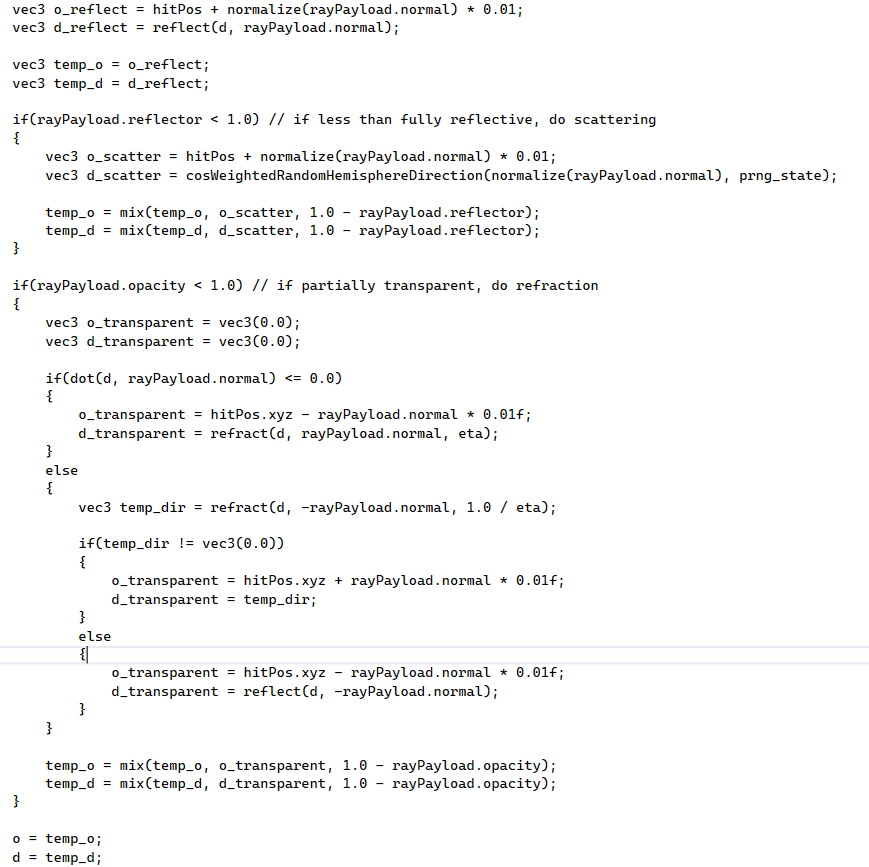
\includegraphics[width = 6 in]{code.png}
  \caption{ Taking transparent objects into consideration.
In essence, instead of always producing a pseudorandom cos-weighted reflection vector, refraction occurs for transparent objects.
}
\end{figure}

\begin{figure} 
\centering
  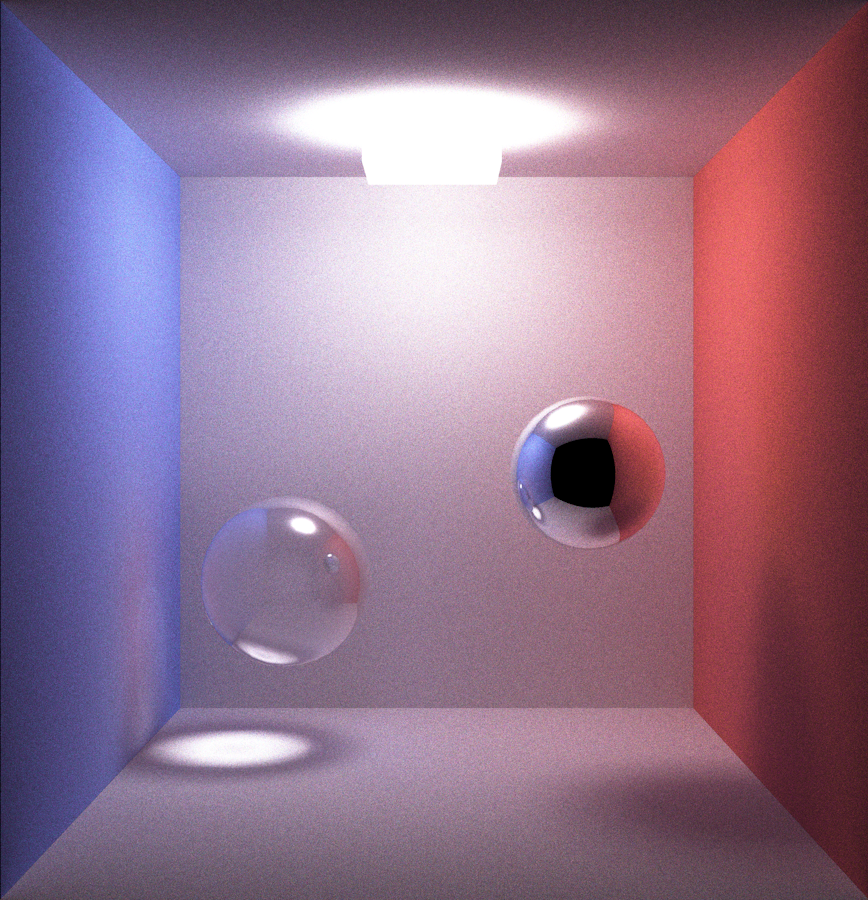
\includegraphics[width = 6 in]{v_rt_reflect_no_chromatic_aberration_low_res.png}
  \caption{ Refraction caustic, without chromatic aberration.
}
\end{figure}


\begin{figure} 
\centering
  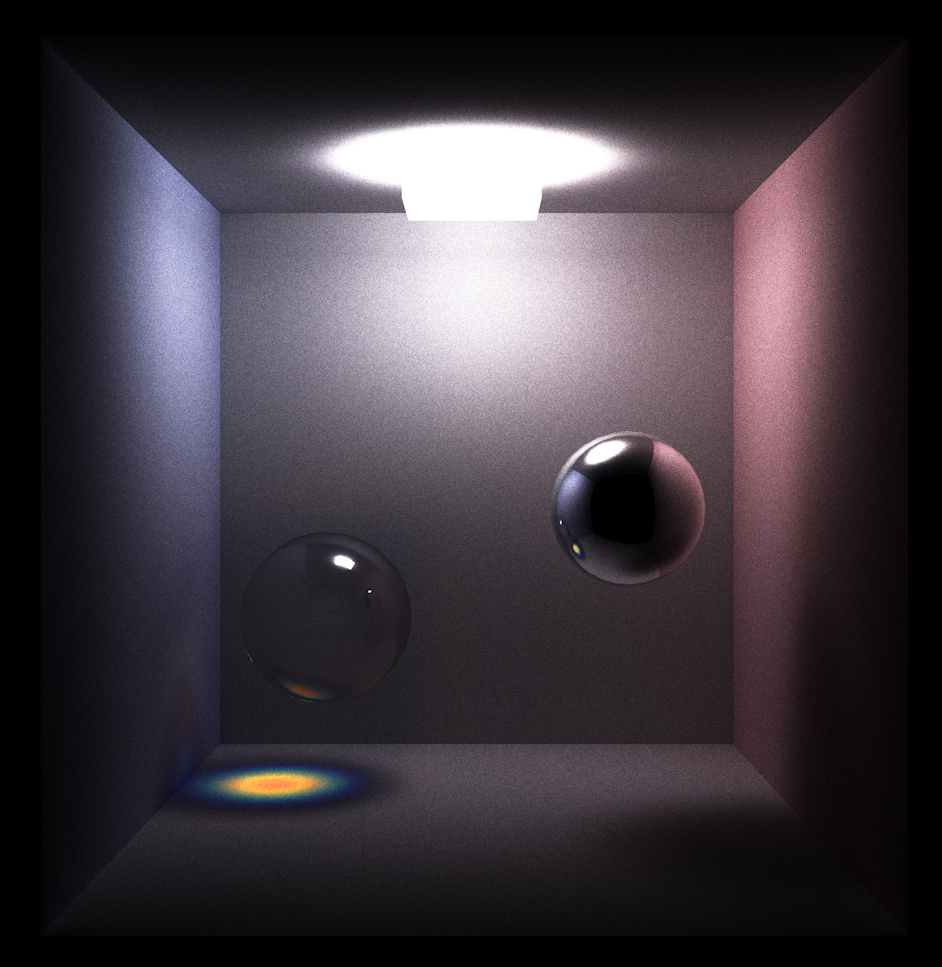
\includegraphics[width = 6 in]{v_rt_reflect_chromatic_aberration_low_res.png}
  \caption{ Refraction caustic, with chromatic aberration.
}
\end{figure}

\begin{figure} 
\centering
  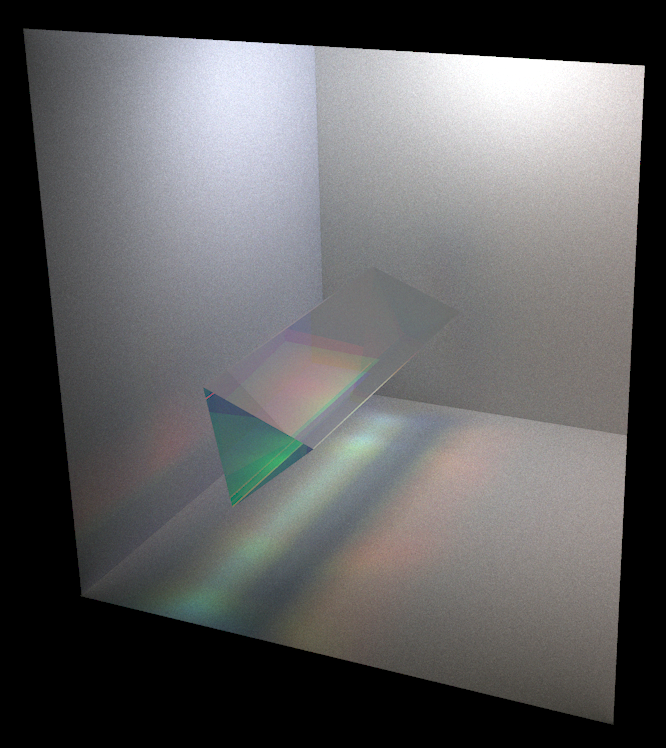
\includegraphics[width = 6 in]{v_rt_reflect_prism.png}
  \caption{ Refraction caustic, with chromatic aberration.
}
\end{figure}

\pagebreak

\begin{thebibliography}{9}

\bibitem{halayka} Halayka. Vulkan code. \url{https://github.com/sjhalayka/cornell_box_textured}
\bibitem{willems1} Willems. Path tracer code. \url{https://github.com/SaschaWillems/VulkanPathTracer}
\bibitem{willems2} Willems. Vulkan demo codes. \url{https://github.com/SaschaWillems/Vulkan}


\end{thebibliography}








\end{document}









